%                                                                 aa.dem
% AA vers. 9.1, LaTeX class for Astronomy & Astrophysics
% demonstration file
%                                                       (c) EDP Sciences
%-----------------------------------------------------------------------
%
%\documentclass[referee]{aa} % for a referee version
%\documentclass[onecolumn]{aa} % for a paper on 1 column  
%\documentclass[longauth]{aa} % for the long lists of affiliations 
%\documentclass[letter]{aa} % for the letters 
%\documentclass[bibyear]{aa} % if the references are not structured 
%                              according to the author-year natbib style

%
% \documentclass[draft]{aa} 
\documentclass{aa}

%
\usepackage{graphicx}
%%%%%%%%%%%%%%%%%%%%%%%%%%%%%%%%%%%%%%%%
\usepackage{txfonts}
%%%%%%%%%%%%%%%%%%%%%%%%%%%%%%%%%%%%%%%%
%\usepackage[options]{hyperref}
% To add links in your PDF file, use the package "hyperref"
% with options according to your LaTeX or PDFLaTeX drivers.
%
\usepackage[]{hyperref}
\hypersetup{colorlinks=true, urlcolor=blue, citecolor=cyan, pdfborder={0 0 0}}

\begin{document} 


\title{An analysis of the most distant catalogued open clusters}
\subtitle{Re-assessing fundamental parameters with Gaia EDR3 and \texttt{ASteCA}}

\author{G. I. Perren\inst{1}
      \and
      M. S. Pera\inst{1}
      \and
      H. Navone\inst{2}
      \and
      R. A. Vázquez\inst{1,3}
      % \fnmsep\thanks{Just to show the usage
      % of the elements in the author field}
}

\institute{Instituto de Astrof\'isica de La Plata (IALP-CONICET), La Plata,
Argentina\\
\email{gabrielperren@gmail.com}
\and
Facultad de Ciencias Exactas, Ingeniería y Agrimensura (UNR-IFIR-CONICET),
Rosario, Argentina
\and
Facultad de Ciencias Astronómicas y Geofísicas (UNLP-IALP-CONICET), 1900 La
Plata, Argentina
% \thanks{The university of heaven temporarily does not
%         accept e-mails}
}
\date{Received September 15, 2021; accepted December 16, 2021}

% \abstract{}{}{}{}{} 
% 5 {} token are mandatory
 
\abstract
% context heading (optional)
% {} leave it empty if necessary  
{Several studies have been presented in the last few years applying some kind of
automatic processing of data to estimate the fundamental parameters of open
clusters. These parameters are later on employed in larger scale analyses, for
example the structure of the Galaxy's spiral arms.
The distance is one of the more straightforward parameters to estimate, yet
enormous differences can still be found among published data. This is
particularly true for open clusters located more than a few Kpc away.}
% aims heading (mandatory)
{
We cross-matched several published catalogues and selected the twenty-five most
distant open clusters ($>$9000 Kpc). We then performed a detailed analysis of
their fundamental parameters, with emphasis on their distances, to determine the
agreement between catalogues and our estimates.}
% methods heading (mandatory)
{Photometric and astrometric data from the Gaia EDR3 survey was employed. The
data was processed with our own membership analysis code (pyUPMASK), and our
package for automatic fundamental cluster's parameters estimation
(\texttt{ASteCA}).}
% results heading (mandatory)
{We find differences in the estimated distances of up to several Kpc
between our results and those catalogued, even for the catalogues that show the
best matches with \texttt{ASteCA} values. Large differences are also found for
the age estimates.}
% conclusions heading (optional), leave it empty if necessary 
{Caution is thus strongly recommended when using catalogued parameters of open
clusters to infer large-scale properties of the Galaxy, particularly for those
located more than a few Kpc away.}

\keywords{
  Methods: statistical --
  Galaxies: star clusters: general --
  (Galaxy:) open clusters and associations: general --
  Techniques: photometric--
  Parallaxes --
  Proper motions
}

\maketitle


\section{Introduction}

 The unprecedented amount of high precision data for parallaxes, proper motions,
 and photometry provided by the Gaia mission in successive
 deliveries~\citep[DR2 and EDR3,][]{Gaia_2016,Gaia_EDR3} offers us a unique
 opportunity to estimate the fundamental parameters, age, distance, the observed
 mass and the metal content of open clusters (OC).
 Indeed, the arrival of new techniques for
 analyzing massive data combined with the increasing data precision promise
 more reliable results than those obtained with the old techniques mostly
 based on the visual inspection of their color-magnitude diagrams and
 isochrone fittings \citep{Phelps1994} or on direct comparison with HR diagrams
 of synthetic clusters \citep{Siess1997}. Automated processes such as the one
 applied by \cite{Kharchenko_2012} have also played an important role in
 determining cluster parameters in a massive way. But the continuous increase
 of high quality data is a defying circumstance where a variety of analysis are
 being considered even including artificial neural networks
 \citep{Cantat_2020} combined with new strategies for determining cluster
 memberships \citep{Krone2014,Cantat2018}.
 %
 The intrinsic value of studying OCs has been profusely described in several
 opportunities and we are not going to repeat them here. However a brief
 enumeration of the importance of these object is appropriate: the oldest OCs
 allow us to investigate the extension in height and radial extension of the
 galactic disk; old OCs tell us about the chemical history, the mixing processes
 and the processes of OCs destruction by interaction with other populations of
 the galaxy as well as the age-metallicity relationship 
 \citep{Friel1995,Tosi2004,Hayes2015}. The youngest OCs, on the other hand, are
 not only used as laboratories to investigate stellar evolution (they allow
 studying in detail the boundary conditions necessary to create new generations
 of stars \citep{Lada2003} but are also routinely employed too in the analysis
 of the Milky Way's
 structure~\citep{Loktin_1992,Moitinho_2006,Vazquez2008,Moitinho_2010}
 becoming particularly useful in the tracing of spiral
 arms~\citep{carraro_2013,Molina_2018}.
 %
 It is unfortunate that young OCs are mainly arranged along the galactic disk
 where the strong visual absorption and the contamination by field stars very
 often prevent observing stars in the lower part of the sequence of these
 objects. In this sense, the situation is not much better at all for the older
 OCs. In fact, these objects do not have very luminous stars in the main
 sequence, although they do in the giant branch. Notwithstanding, stars in the
 lower part of their sequences as well as those ones belonging to the giant
 branch share similar photometric characteristics with field stars making
 difficult to unravel to which population each star belongs~\citep{Hayes2015}.
 %
 The situation worsens as the distance to the older OCs increases because the
 limiting magnitude increases, which results in only a small portion of
 the lower part being usually divisible. But it is not only the photometric
 space that is disturbed by distance. The proper motions of far OCs are
 extremely difficult to separate clearly from those characterizing the field
 population against which we see them projected, therefore introducing an
 additional degree of confusion in determining memberships.

 Our interest in this current article is twofold. On the one hand, it is focused
 on reexamining the distances and properties of the most distant OCs cataloged
 so far in our Galaxy. A total of 25 such distant clusters were found
 inspecting four different recognized databases that satisfy this requirement as
 we will explain below. However, these bases show enormous differences in the
 parameters determined for them, both in distances and in ages. In part, the
 differences in the parameters for the same object may be
 due to the different techniques used to obtain them combined with the problem
 of the very large distance at which they are located.
 %
 It is of great interest that the ages for most of these OCs included in recent
 catalogs, estimated with advanced analysis techniques, are presumed to be
 larger than one billion years. But in other catalogs these same clusters have
 relatively small ages and shorter distances as well. We want to
 contribute with our analysis to resolve the origin of these differences.
 %
 On the other hand, we want to test our new membership estimation technique
 pyUPMASK~\citep{Pera_2021} in combination with
 \texttt{ASteCA}~\citep{Perren_2015}, on clusters with proper motions that are
 not easily distinguishable from that of surrounding stars, made up by a small
 number of members, and with non-trivial sequences in the photometric space.\\


 This article is structured as follows. In Sect~\ref{sec:cat_clust_data} we
 introduce the stellar cluster catalogues, the clusters selected to be
 analyzed (crossed-matched from those catalogues), and the photometric and
 astrometric data used to perform the analysis. Sect~\ref
 {sec:clust_analy} presents the methods employed in the study of all the
 clusters. The comparison of the estimated parameters with the catalogued
 values for each cluster is done in Sect~\ref{sec:results}. Finally,
 conclusions are highlighted in Sect~\ref{sec:conclusions}.





% =============================================================================
\section{Catalogues, clusters, and data}
 \label{sec:cat_clust_data}

 We selected four catalogues to cross-match and subsequently identify the most
 distant clusters: \citet[][New Catalog of Optically Visible Open Clusters and
 Candidates, hereinafter OC]{Dias_2002},~\citet[][WEBDA,\footnote{
 \url{https://webda.physics.muni.cz/}} hereinafter WB]{Netopil_2012},
 \citet[][Milky Way Star Clusters Catalog, hereinafter MW]{Kharchenko_2012},
 and~\citet[][hereinafter CG]{Cantat_2020}.
 %
 The first two (OC and WB) are compilations of open clusters' fundamental
 parameters from the literature. They contain around 1700 (WB) and 2100 
 (OC) entries, and are heavily used in the field of open cluster research.
 The parameter values in both catalogues are heterogeneous, being compiled from
 various sources.
 The MW catalog is the largest one ($\sim$3000 entries) and, similarly to the CG
 catalog ($\sim$2000 entries), is composed of homogeneous fundamental parameter
 values obtained for all its entries. The method employed by the authors of the
 MW catalog is a semi-automated isochrone fit, while the CG catalog was
 generated employing an artificial neural network (trained on parameter values
 taken from the literature).

 Since we are interested in the open clusters most distant from the Sun, we
 select from these cross-matched catalogues those that are located at a
 distance of 9000 pc or more in either of them. This is an arbitrary value that
 results in enough clusters to draw general conclusions, but not too many that
 would impede their detailed analysis.\\

 The initial full list consisted of thirty-eight open clusters. Eleven of these
 were found only in the MW catalog with distances larger than 9000 pc. These are
 either listed with substantially smaller distances in the other catalogs, or
 too sparse and or dubious. Hence these clusters were removed from the
 cross-matched list.
 %
 Two other clusters were also removed: Shorlin 1 ($\alpha_{2000}$=166.44,
 $\delta_{2000}$=-61.23) and FSR0338
 ($\alpha_{2000}$=327.93, $\delta_{2000}$=55.33). The latter appears in WB and
 MW at a distance of 12600 pc and 5600 pc respectively, while the former is
 listed only in MW with a distance of 14655 pc. Shorlin1 is studied
 in~\cite{Carraro_2009} and~\cite{Turner_2012}; in both cases the authors
 conclude that this is not a real cluster but a grouping of young stars.
 % Shorlin 1
 %
 % Carraro & Costa (2009)
 % > We also present evidence that this extremely distant group, formerly assumed
 % to be a star cluster (Shorlin 1), is a diffuse, young population, typically
 % found in spiral galaxies.
 %
 % Turner (2012)
 % > ...star counts also imply that Shorlin 1 is unlikely to represent a true
 % cluster, but is instead merely the trapezium-like remains of a previously-
 % bound cluster with an implied age of only a few Myr, according to the likely
 % presence of O-type stars within its boundaries.
 %
 FSR0338 is analyzed in~\cite{Froebrich_2010} where a distance of 6000 pc is
 assigned, but with large uncertainties.
 % Froebrich et al. (2010)
 % > Th high probability members of this newly identified cluster seem to indicate
 % an object with an age of 0.4 Gyrs at a distance of 6 kpc. The scatter in the
 % data points suggests larger than normal uncertainties for the parameters.
 %
 In both cases we find no evidence of a true stellar cluster in these regions.
 We base our conclusion on two findings. First, the large proper motions
 dispersion of the stars that occupy the overdensity around the central
 coordinates assigned to either object. Second, the lack of a clear sequence in
 their respective color-magnitude diagrams (CMD). These two clusters are thus
 discarded from further analysis. The remaining twenty-five clusters that will
 be studied in this work are shown in Table~\ref{tab:clusters}. Most of the
 selected clusters are located in the Third Quadrant with all of them in the
 latitude range of [-12$^{\circ}$, 8$^{\circ}$], relatively close to the
 galactic plane. The final list thus contains 24 clusters in the MW catalog,
 21 in WB, 19 in OC, and 16 in CG.

 \begin{table*}
 \caption{Selected open clusters with a catalogued distance $\geq$9000 pc,
 ordered by right ascension. The ages are expressed as the logarithm, and the
 distances are in parsec. In parenthesis, the short names used for the clusters
 throughout the article. Clusters with no distances below the 9000 pc limit in
 any of the catalogs are marked with boldface.}
 \label{tab:clusters}
 \centering
 \begin{tabular}{lllllllllll}
 \hline\hline
 Cluster & $\alpha_{2000}$  & $\delta_{2000}$ & OC$_{age}$ & OC$_{dist}$ & CG$_{age}$ &
 CG$_{dist}$ & WB$_{age}$ & WB$_{dist}$ & MW$_{age}$ & MW$_{dist}$ \\
 \hline
 Berkeley 73 (BER73)     & 95.5   & -6.35     & 9.18  & 9800  & 9.15  & 6158  &
 9.36 & 6850 & 9.15  & 7881  \\
 Berkeley 25 (BER25)     & 100.25 & -16.52    & 9.7   & 11400 & 9.39  & 6780  &
 9.6   & 11300 &  9.7   & 11400 \\
 Berkeley  75 (BER75)     & 102.25 & -24       & 9.6   & 9100  & 9.23  &  8304 
 & 9.48  & 9800  & 9.3   & 6273  \\
 Berkeley  26 (BER26)     & 102.58 & 5.75      & 9.6   & 12589 & -   & -   & 9.6
 & 4300  & 8.71  & 2724  \\
 Berkeley  29 (\textbf{BER29})     & 103.27 & 16.93     & 9.025 & 14871 & 9.49  & 12604 &
 9.025 & 14871 & 9.1   & 10797 \\
 Tombaugh 2 (TOMB2)     & 105.77 & -20.82    & 9.01  & 6080  & 9.21  & 9316  &
 9.01 & 13260 & 9.01  & 6565  \\
 Berkeley 76 (BER76)     & 106.67 & -11.73    & 9.18  & 12600 & 9.22  & 4746  &
 9.18 & 12600 & 8.87  & 2360  \\
 FSR 1212 (F1212)   & 106.94 & -14.15    & -   & -   & 9.14  & 9682  & -   & -
 & 8.65  & 1780  \\
 Saurer 1 (\textbf{SAU1})   & 110.23 & 1.81      & 9.7   & 13200 & -   & -   & 9.85  &
 13200 & 9.6   & 13719 \\
 Czernik 30 (CZER30)    & 112.83 & -9.97     & 9.4   & 9120  & 9.46  & 6647  &
 9.4 & 6200  & 9.2   & 6812  \\
 Arp-Madore 2 (\textbf{ARPM2})     & 114.69 & -33.84    & 9.335 & 13341 & 9.48  & 11751 &
 9.335 & 13341 & 9.335 & 13338 \\
 vd Bergh-Hagen 4 (\textbf{BH4})     & 114.43 & -36.07    & -   & -   & -   & -  
 & 8.3   & 19300 & -   & -   \\
 FSR 1419 (F1419)   & 124.71 & -47.79    & -   & -   & 9.21  & 11165 & -   & -   & 8.375 & 7746  \\
 vd Bergh-Hagen 37 (BH37)    & 128.95 & -43.62    & 8.84  & 11220 & 8.24 
 & 4038  & 8.85  & 2500  & 7.5   & 5202  \\
 ESO 092 05 (E9205)  & 150.81 & -64.75    & 9.3   & 5168  & 9.65  & 12444 &
 9.78  & 10900 & 9.3   & 5168  \\
 ESO 092 18 (E9218)  & 153.74 & -64.61    & 9.024 & 10607 & 9.46  & 9910  &
 9.024 & 607   & 9.15  & 9548  \\
 Saurer 3 (SAU3)   & 160.35 & -55.31    & 9.3   & 9550  & -   & -   & 9.45  &
 8830 & 9.3   & 7075  \\
 Kronberger 39 (KRON39)    & 163.56 & -61.74    & -   & 11100 & -   & -   & -   &
 -   & 6     & 4372  \\
 ESO 093 08 (E9308)  & 169.92 & -65.22    & 9.74  & 14000 & -   & -   & 9.65  &
 3700  & 9.8   & 13797 \\
 vd Bergh-Hagen 144 (BH144)   & 198.78 & -65.92    & 8.9   & 12000 & 9.17
 & 9649  & 8.9   & 12000 & 9     & 7241  \\
 vd Bergh-Hagen 176 (BH176)   & 234.85 & -50.05    & -   & -   & -   & - 
 & -   & 13400 & 9.8   & 18887 \\
 Kronberger 31 (\textbf{KRON31})    & 295.05 & 26.26     & -   & 11900 & -   & -   & -   &
 -   & 8.5   & 12617 \\
 Saurer 6 (SAU6)   & 297.76 & 32.24     & 9.29  & 9330  & -   & -   & 9.29  &
 9330 & 9.2   & 7329  \\
 Berkeley 56 (\textbf{BER56})     & 319.43 & 41.83     & 9.6   & 12100 & 9.47  & 9516  &
 9.6 & 12100 & 9.4   & 13180 \\
 Berkeley 102 (BER102)    & 354.66 & 56.64     & 9.5   & 9638  & 9.59  & 10519 &
 8.78  & 2600  & 9.14  & 4900 \\
 \hline
 \end{tabular}
 \end{table*}

 There are two other major works where a large catalog of analyzed open clusters
 is presented: \cite{Lui_2019} and \cite{Dias_2021}. The latter does not contain
 clusters with such large distances, and was hence not used. The former lists
 only four clusters that are also present in our set of twenty-five selected
 clusters. None of their distances comply with our selection filter, hence this
 database was not included. This fact notwithstanding, their distance values will
 be mentioned in the discussion of the results in Sect.~\ref{sec:results}.\\

 Data from Gaia EDR3~\citep{Gaia_2016,Gaia_EDR3} was retrieved for a box of 20
 arcmin of length around the central coordinates for all the clusters. We
 employed equatorial coordinates, parallax, proper motions, and photometry
 ($G$, $(G_{BP}-G_{RP})$) from these survey.
 %
 In Fig~\ref{fig:MWmap} we show the twenty-five selected clusters for each of
 the four catalogues, positioned on the face-on view of the Galaxy (top), and
 two edge on views (center, bottom). The spiral arms are those presented
 in~\cite{Momany_2006}. The large dispersion for the distances
 assigned to each cluster in different catalogs is clearly visible, where
 ideally the position of all the clusters would overlap for the four catalogs.\\

 In what follows we will only show the figures for a single representative
 cluster (Berkeley 29) to avoid the clutter and improve the readability of the
 article. The plots for the remaining clusters can be found in the appendix.

 \begin{figure*}
  \resizebox{\hsize}{!}{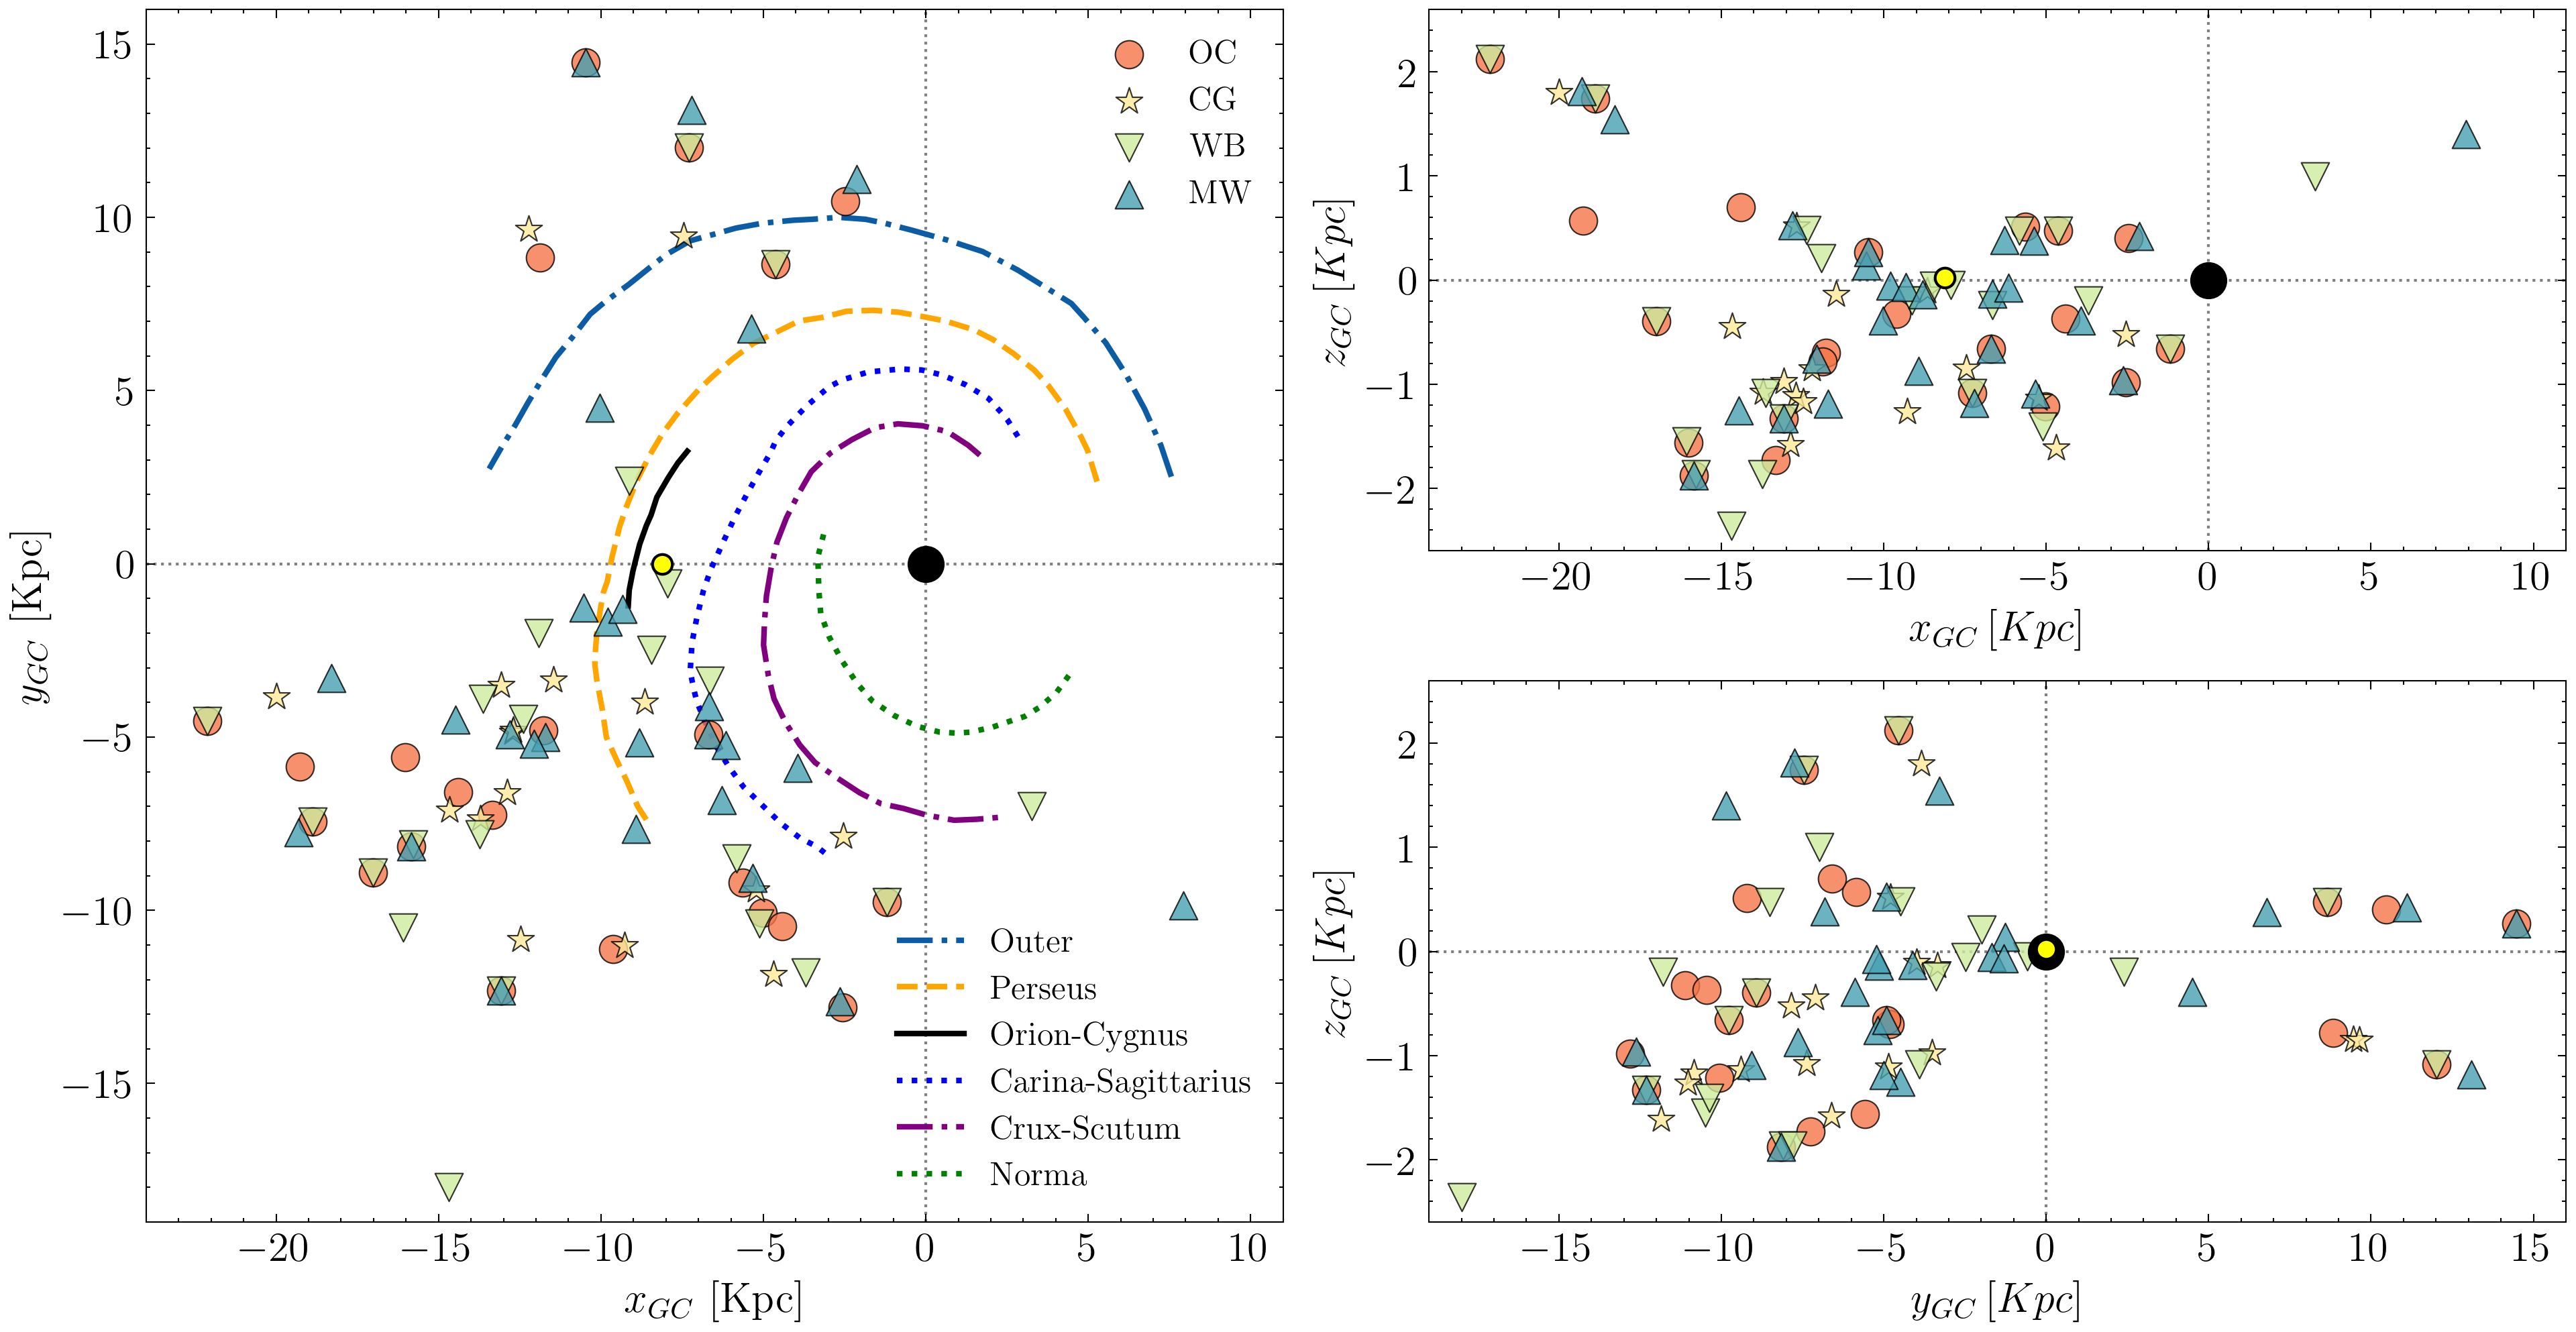
\includegraphics[]{figs/MWmap.png}}
  \caption{Right: position of the twenty-five clusters selected from the four
  catalogs mentioned in the text, on a face-on view of the Milky Way. The Sun
  and the center of the Galaxy are marked with a yellow filled circle and a
  black filled circle, respectively. Top and bottom left: edge-on views, same
  color and marker conventions as above.}
  \label{fig:MWmap}
 \end{figure*}





% =============================================================================
\section{Cluster analysis}
 \label{sec:clust_analy}

 \subsection{Structural analysis}
  \label{sec:clust_analy}

  The first step in the cluster analysis is the estimation of their structural
  properties, i.e. center coordinates and limiting radius. Although centers and
  diameters are present in (some of) the catalogues, not all of these values are
  correct. We use our \texttt{ASteCA} package
  \citep{Perren_2015}\footnote{\url{http://asteca.github.io/}} throughout this
  work to perform the structural and fundamental parameters analysis. We have
  applied this tool to the study of hundreds of clusters in previous articles,
  with excellent results~\citep{Perren_2017,Perren_2020}.

  The center values are obtained applying a two-dimensional kernel density
  analysis (KDE) on each of the cluster's coordinates. This method assigns the
  center of the cluster to the point with the largest density in the frame. A
  King's profile~\citep{King_1962} fit is then performed on the radial density
  profile of each cluster to estimate their core and tidal radii ($r_{c}$,
  $r_{t}$). The adopted radius $r_{a}$ is the limiting distance from the
  center used to define the studied cluster region for each cluster. These
  values are shown in Table~\ref{tab:radii}. The adopted radius in this work is
  on average 50\% smaller than the tidal radius. This decision allows us to
  alleviate the issue of field star contamination, while ensuring that only a
  small number of true members (cluster stars located as far from the
  center as the tidal radius) are lost. The fraction of lost members can be
  estimated integrating the King's profile. This fraction depends on the
  concentration of the cluster ($r_{t}/r_{c}$) and the value of the adopted
  radius as a fraction of the tidal radius ($r_{a}/r_{t}$). In our case, less
  than 20\% of the members could be lost in a worst case scenario. Since these
  are clusters that are strongly contaminated (particularly in the parallax and
  proper motions spaces), the trade off between losing a small portion of
  members and improving the contrast of the true members over the field noise,
  is positive.

  The restrictive $r_{a}$ values used in our analysis means that the total
  estimated mass for each cluster shown in Sect.~\ref{sec:results}, must be
  thought of as a lower limit.\\

  \begin{table}
  \caption{Core ($r_{c}$), tidal ($r_{t}$), and adopted ($r_{a}$) radii values.
  The first two are shown with their respective 16th an 84th percentiles in
  parenthesis.}
  \label{tab:radii}
  \centering
  \begin{tabular}{llll}
  \hline\hline
  Cluster & $r_{c}$ (16th, 84th) &  $r_{t}$ (16th, 84th) & $r_{a}$\\
  \hline
   BER73         & 0.6 (0.5, 0.7) &  4.9 (3.8, 6.3) &  2.0\\
   BER25         & 1.5 (1.2, 1.8) &  7.0 (6.2, 8.0) &  5.0\\
   BER75         & 0.4 (0.3, 0.5) &  5.0 (3.6, 6.6) &  2.0\\
   BER26         & 0.7 (0.5, 1.0) &  3.4 (2.5, 4.5) &  1.6\\
   BER29         & 0.5 (0.4, 0.5) &  7.4 (6.4, 8.6) &  3.0\\
   TOMB2         & 0.9 (0.8, 0.9) &  6.7 (6.1, 7.4) &  3.5\\
   BER76         & 1.6 (1.2, 2.5) &  7.4 (5.7, 9.6) &  4.0\\
   F1212         & 0.8 (0.6, 1.1) &  8.8 (6.6, 10.7) & 3.0\\
   SAU1          & 0.7 (0.5, 1.0) &  3.9 (2.9, 5.4) &  2.0\\
   CZER30        & 0.6 (0.4, 0.7) &  6.4 (4.8, 8.2) &  2.5\\
   ARPM2         & 1.4 (1.0, 2.0) &  4.1 (3.4, 4.9) &  3.0\\
   BH4           & 0.4 (0.3, 0.5) &  5.7 (4.0, 7.1) &  2.0\\
   F1419         & 1.2 (0.9, 1.8) &  6.0 (4.3, 8.3) &  3.0\\
   BH37          & 1.2 (0.8, 1.9) &  3.8 (2.5, 5.6) &  2.0\\
   E9205         & 1.0 (0.9, 1.3) &  4.4 (3.7, 5.3) &  3.0\\
   E9218         & 0.6 (0.6, 0.7) &  6.5 (5.9, 7.3) &  3.0\\
   SAU3          & 0.5 (0.4, 0.6) &  4.9 (3.8, 6.4) &  2.0\\
   KRON39        & 0.3 (0.2, 0.3) &  5.6 (4.1, 7.0) &  2.0\\
   E9308         & 0.2 (0.2, 0.2) &  5.0 (4.2, 5.7) &  1.5\\
   BH144         & 0.3 (0.3, 0.4) &  2.8 (2.3, 3.4) &  1.5\\
   BH176         & 0.6 (0.5, 0.7) &  4.6 (3.8, 5.8) &  2.0\\
   KRON31        & 0.5 (0.4, 0.6) &  6.9 (5.7, 7.6) &  2.0\\
   SAU6          & 0.5 (0.4, 0.7) &  3.7 (2.9, 4.8) &  2.0\\
   BER56         & 1.6 (1.4, 1.7) &  8.1 (7.4, 8.9) &  4.5\\
   BER102        & 1.0 (0.8, 1.5) &  3.8 (3.0, 4.9) &  2.5\\
   % BER73         & 0.6$_{0.5}^{0.7}$ &  4.9$_{3.8}^{6.3}$ &  2.0\\
   % BER25         & 1.5$_{1.2}^{1.8}$ &  7.0$_{6.2}^{8.0}$ &  5.0\\
   % BER75         & 0.4$_{0.3}^{0.5}$ &  5.0$_{3.6}^{6.6}$ &  2.0\\
   % BER26         & 0.7$_{0.5}^{1.0}$ &  3.4$_{2.5}^{4.5}$ &  1.6\\
   % BER29         & 0.5$_{0.4}^{0.5}$ &  7.4$_{6.4}^{8.6}$ &  3.0\\
   % TOMB2         & 0.9$_{0.8}^{0.9}$ &  6.7$_{6.1}^{7.4}$ &  3.5\\
   % BER76         & 1.6$_{1.2}^{2.5}$ &  7.4$_{5.7}^{9.6}$ &  4.0\\
   % F1212         & 0.8$_{0.6}^{1.1}$ &  8.8$_{6.6}^{10.7}$ & 3.0\\
   % SAU1          & 0.7$_{0.5}^{1.0}$ &  3.9$_{2.9}^{5.4}$ &  2.0\\
   % CZER30        & 0.6$_{0.4}^{0.7}$ &  6.4$_{4.8}^{8.2}$ &  2.5\\
   % ARPM2         & 1.4$_{1.0}^{2.0}$ &  4.1$_{3.4}^{4.9}$ &  3.0\\
   % BH4           & 0.4$_{0.3}^{0.5}$ &  5.7$_{4.0}^{7.1}$ &  2.0\\
   % F1419         & 1.2$_{0.9}^{1.8}$ &  6.0$_{4.3}^{8.3}$ &  3.0\\
   % BH37          & 1.2$_{0.8}^{1.9}$ &  3.8$_{2.5}^{5.6}$ &  2.0\\
   % E9205         & 1.0$_{0.9}^{1.3}$ &  4.4$_{3.7}^{5.3}$ &  3.0\\
   % E9218         & 0.6$_{0.6}^{0.7}$ &  6.5$_{5.9}^{7.3}$ &  3.0\\
   % SAU3          & 0.5$_{0.4}^{0.6}$ &  4.9$_{3.8}^{6.4}$ &  2.0\\
   % KRON39        & 0.3$_{0.2}^{0.3}$ &  5.6$_{4.1}^{7.0}$ &  2.0\\
   % E9308         & 0.2$_{0.2}^{0.2}$ &  5.0$_{4.2}^{5.7}$ &  1.5\\
   % BH144         & 0.3$_{0.3}^{0.4}$ &  2.8$_{2.3}^{3.4}$ &  1.5\\
   % BH176         & 0.6$_{0.5}^{0.7}$ &  4.6$_{3.8}^{5.8}$ &  2.0\\
   % KRON31        & 0.5$_{0.4}^{0.6}$ &  6.9$_{5.7}^{7.6}$ &  2.0\\
   % SAU6          & 0.5$_{0.4}^{0.7}$ &  3.7$_{2.9}^{4.8}$ &  2.0\\
   % BER56         & 1.6$_{1.4}^{1.7}$ &  8.1$_{7.4}^{8.9}$ &  4.5\\
   % BER102        & 1.0$_{0.8}^{1.5}$ &  3.8$_{3.0}^{4.9}$ &  2.5\\
  \hline
  \end{tabular}
  \end{table}

  In Fig.~\ref{fig:BER29_struct} we show the center and radii estimation
  processes for the cluster Berkeley 29.

  \begin{figure*}
   \resizebox{\hsize}{!}{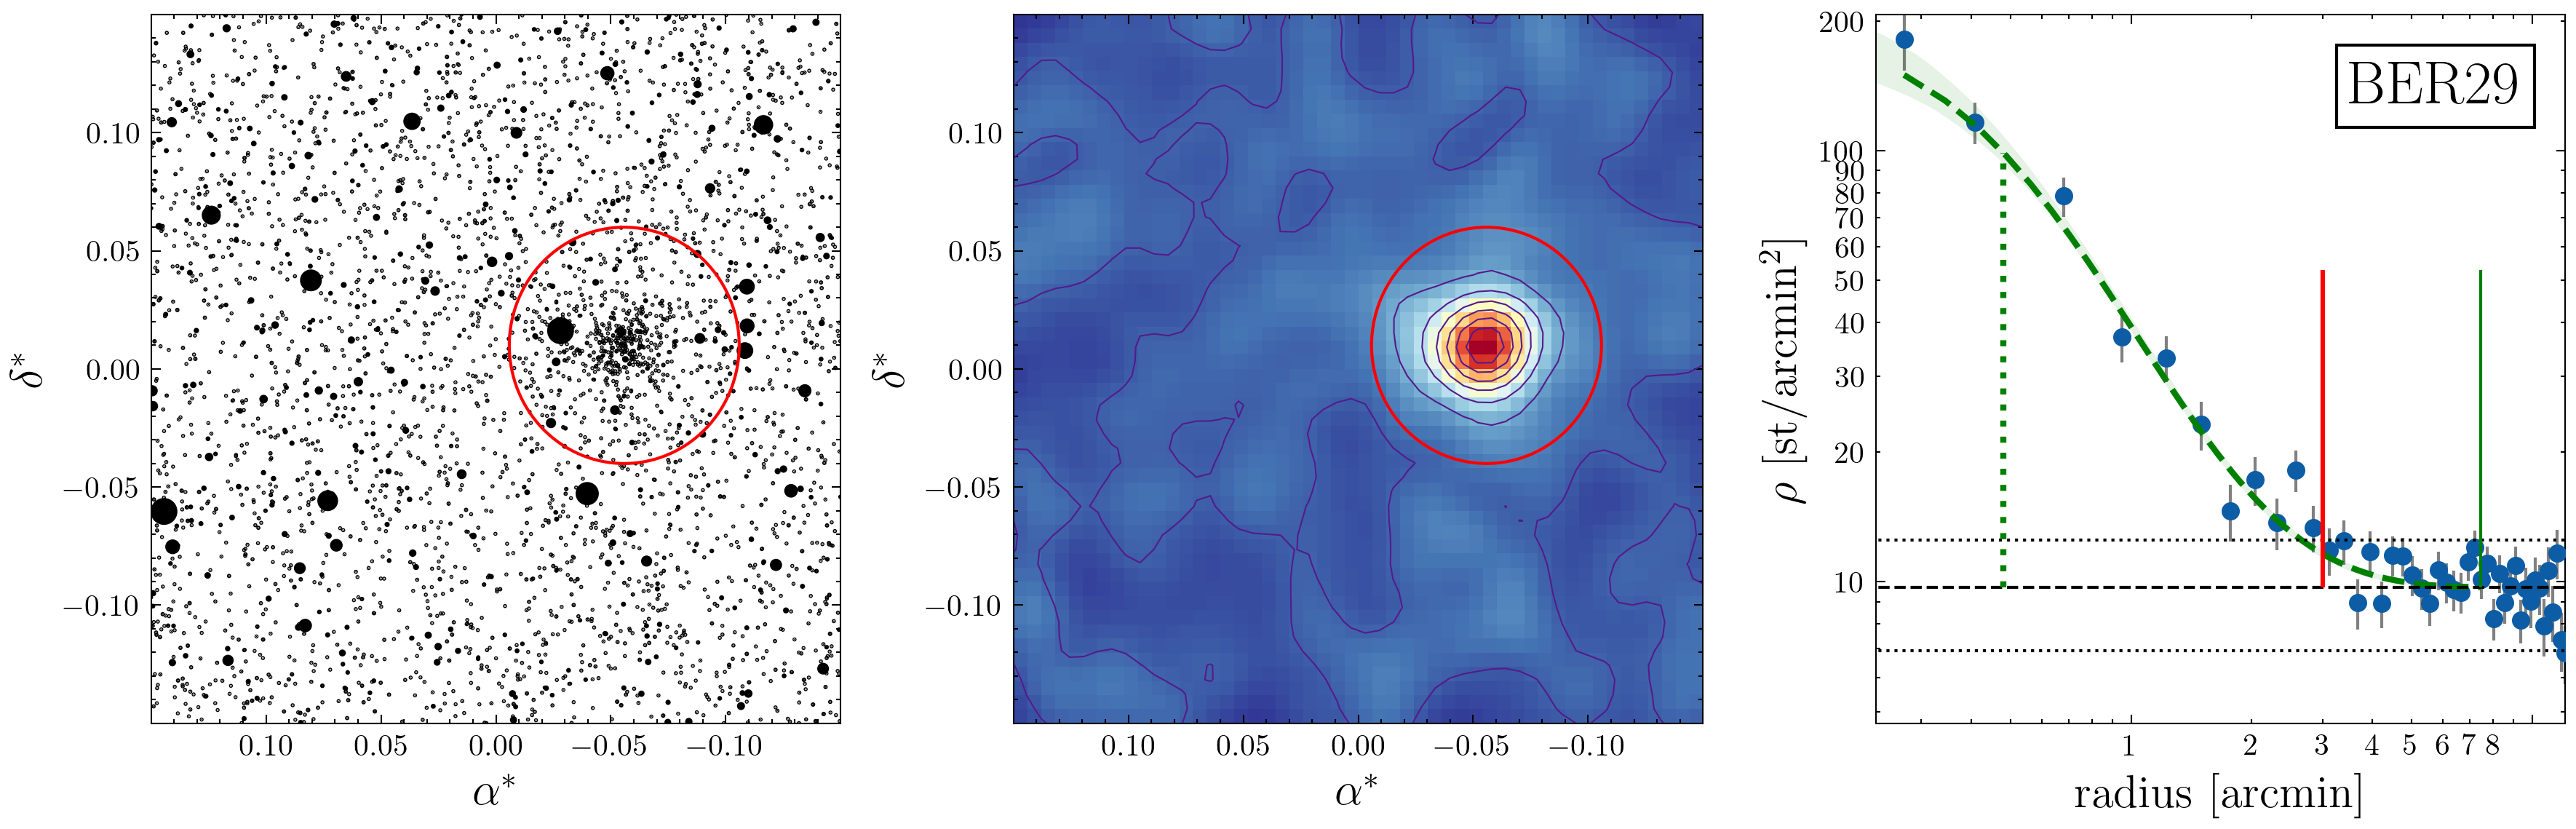
\includegraphics[]{figs/BER29_struct.png}}
   \caption{Structural analysis of the cluster Berkeley 29. Left: analyzed
   20x20 arcmin frame with the estimated cluster region enclosed in a red circle.
   The asterisks in the equatorial coordinates indicate that these were shifted
   and transformed so that the center of the frame is located at (0, 0) and to
   remove projection artifacts. Center:
   same frame but shown as as two-dimensional density map. Right: radial density
   plot (logarithmic axis). The dashed green line and the shaded green area are
   the King profile fit and its 16th-84th uncertainty region, respectively. The
   green dotted vertical line, solid red vertical line, and solid green vertical
   line, are the core, adopted, and tidal radii, respectively. The dashed and
   dotted horizontal black lines are the field density estimate and its $\pm
   1\sigma$ region, respectively.}
   \label{fig:BER29_struct}
  \end{figure*}


 \subsection{Fundamental parameters}
  \label{ssec:fund_pars}

  membership here

  \begin{figure*}
   \resizebox{\hsize}{!}{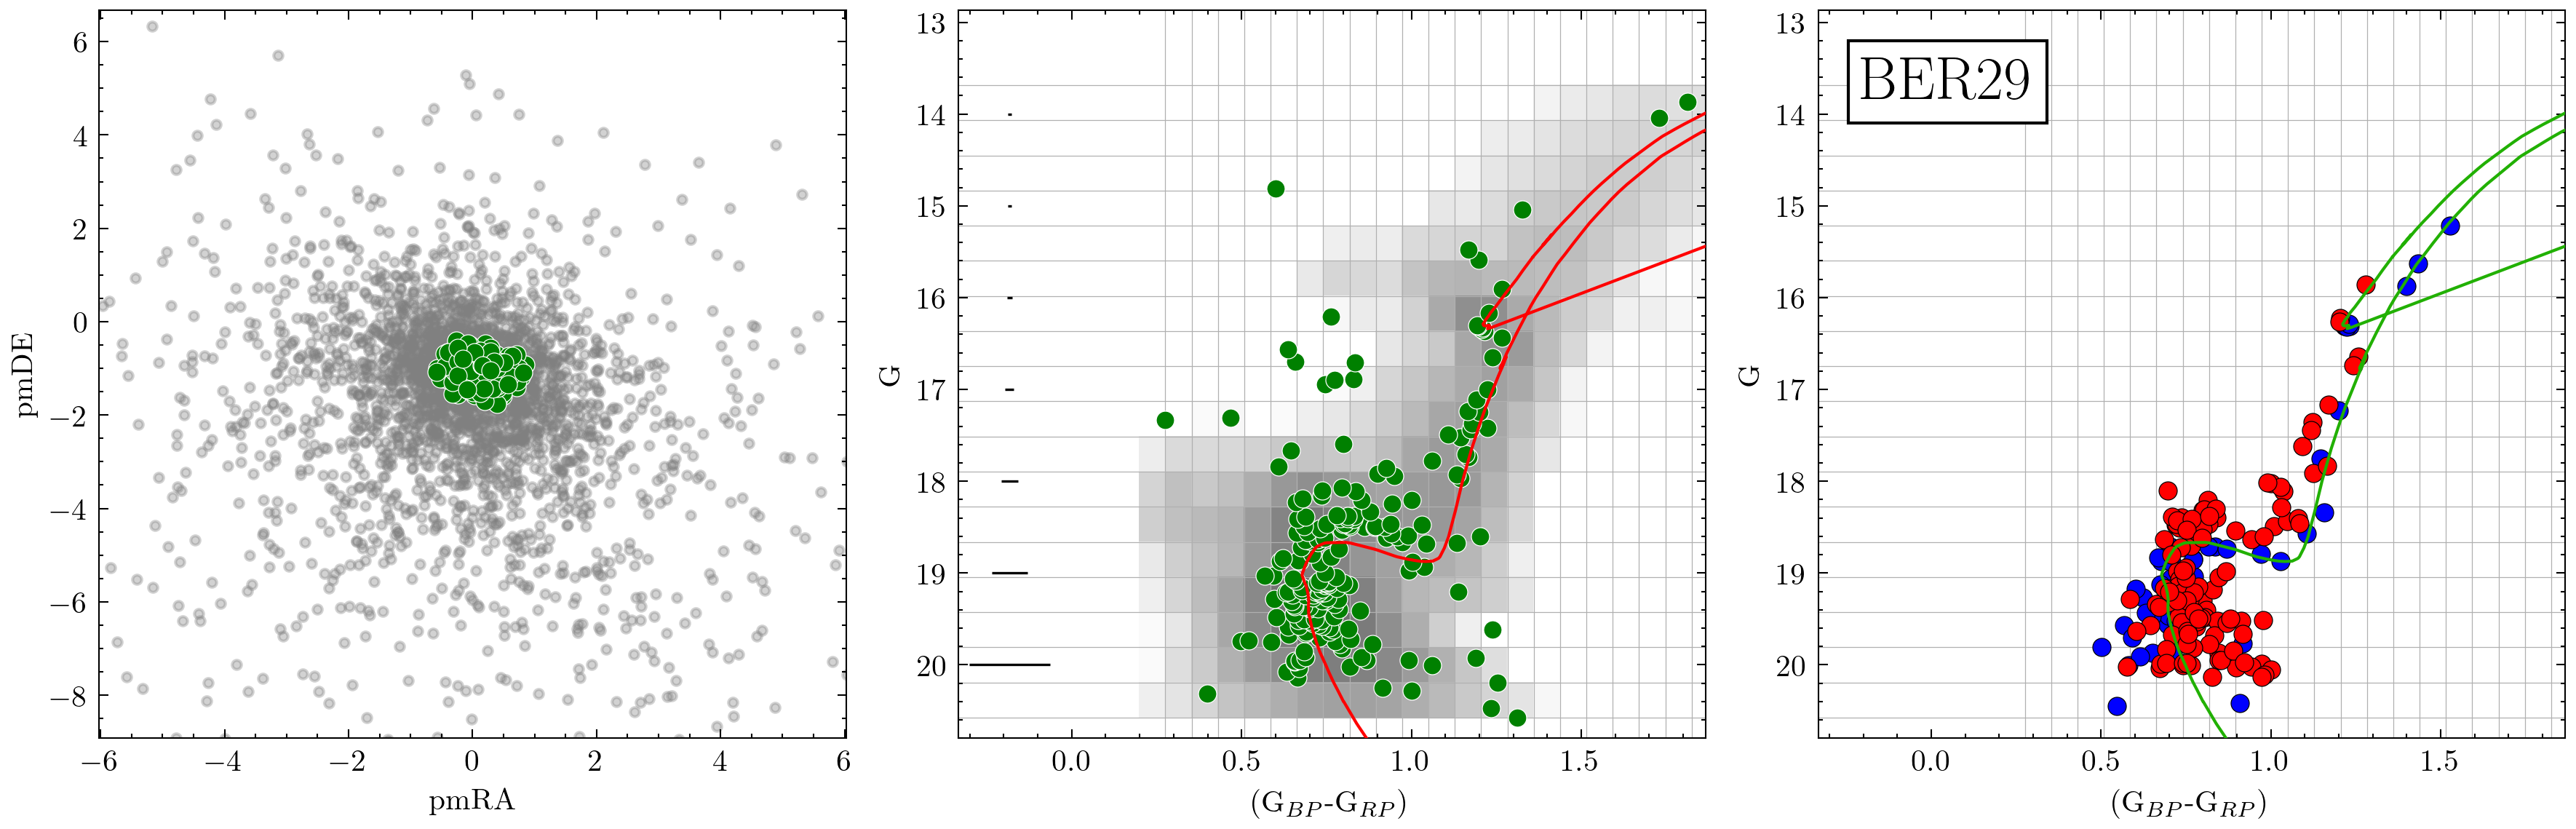
\includegraphics[]{figs/BER29_fpars.png}}
   \caption{xxx}
   \label{fig:BER29_fpars}
  \end{figure*}





% =============================================================================
\section{Discussion and results}
 \label{sec:results}

\textbf{Saurer 3}:
The color magnitude diagram (CMD hereinafter) of this cluster suggests a ''turn-off'' point (TO from now on) at about G=19. Members appear scattered around the main sequence, probably because of increasing of Gaia photometry errors with distance. The evident cluster ''red-clump'', RC hereinafter, is set at G= 16.5. The analysis gives a distance 6.7 kpc and the age is 4.8 Gyr. \cite{2003MNRAS.346...18C} utilize CCD VI photometry finding a distance of 9.6 kpc, over 50\% above our estimate. The age they assigned, 1.8 Gyr, too much different from ours as well. Maybe these differences in age and distance come from wrong membership assignations when using photometric arguments in a zone of confusion between cluster and background stars. 

\textbf{Saurer 6}:
The CMD denotes a wide and short main sequence where the TO appears at few more than G=18. The giant branch is quite scattered though the RC is evident. The RDP gives a cluster radius of $2^{\prime}$ showing high star density what may explain the main sequence widening. Also duplicity of stars is a quite reasonable assumption. Saurer 6 is 1.6 Gyr old and its distance is 8.74 kpc. This object also was studied by \cite{2002AJ....123.2552F} using CCD VI photometry. For them, Saurer 6 is about 2 Gyr old and is placed at 9.3 kpc, both values are not far from ours and neither is the color excess E they found.

\textbf{Berkeley 102}:
 The CMD is composed of a scattered main sequence with the TO at G=18.5 and a defined giant branch next. Some stars above the TO could be binary stars or unresolved pairs. This cluster is placed at 7.6 kpc and is 4.9 Gyr old. Both age and distance are strongly discrepant with \cite{Cantat_2020} values since they give a distance of 10.5 kpc and an age near 3.9 Gyr. The nature of the analysis done by \cite{Cantat_2020} makes difficult explain the different results despite data are the same. There is a small color excess discrepancy between our analysis and that of CG that cannot reduce the gap between results. Certainly, when looking at the CMD, one is led to think that the TO could be set at G=18 instead of G=18.5, but this would end up in an even shorter distance and therefore larger discrepancy with CG.  

\textbf{Berkeley 25}:
The CMD shows several stars above the TO that are candidates to blue straggler stars. The cluster giant branch is well evident. The RDP of Berkeley 25 shows that this cluster has a radius about $5^{\prime}$; the distance we found is 7.2 kpc and the color excess is 0.35. The cluster age is 5.6 Gyr. These values are quite different from the estimated ones by \cite{2005A&A...442..917C} who found that Berkeley 25 is 3.0 Gyr old, its color excess is E=0.17 and the distance is d=11.3 kp (four kpc over our estimate). It is to be added that the radius Of Berkeley 25 given by these authors is $0.8^{\prime}$, just a 20\% of the found here. No doubt, part of the disagreement arise from a better estimation of the cluster parameters with Gaia data.  Berkeley 25 was included in the Dias et al catalog with a distance of 11.4 kpc and an age of 5.0 Gyr.

\textbf{Berkeley 26}:
It is not so relevant projected against the background field. Although the cluster RDP is well established and the radius is near $2^{\prime}$, the TO is confuse due to the scatter of the stars and the likely presence blue straggler candidates. The giant branch is less notorious so that the best synthetic cluster fitting at the position of the TO results in a  E= 0.45, is located at d= 4.8 kp and is 7.7 Gys old. \cite{2010MNRAS.402.2720P} investigated this object previously finding  E=0.75, age= 4 Gyr and d=4.3 kpc. The differences in excess and distance can be justifiable in terms of the small number of stars and difficulties when estimating photometric membership alone. Also the age difference is huge; we understand that this difference may be due to the fact that we set the cluster TO at G=18.5, almost half a magnitude below the used by Piatti et al. This cluster has been included in the Dias et al catalog with a distance of 12.5 kpc -that is why we included it in our study-, probably a mistake.


\textbf{Berkeley 76}:
The CMD of Berkeley 76 shows a diffuse TO at G=16.5 followed by a relevant giant branch. The parameters indicate a distance of 5.3 kpc, an age of 1.9 Gyr and a color excess of 0.58. There is a strong disagreement with the distance given by \cite{2013MNRAS.428..502C} since their TO is at V=18.5, almost 2 mag below ours and the distance they found is 12.6 kpc with about $2.5^{\prime}$ radius (the RDP provides a radius over $4^{\prime}$) and 1.5 Gyr old. Only the a E=0.55 and the cluster age are similar to our values. We believe that the distance difference with Carraro et al. comes from a wrong TO adopted by Carraro et al., due to the difficulties in determining cluster membership using just photometric arguments. Our results, on the other hand, are not very different from the ones obtained by \cite{Cantat_2020}. 


\textbf{CZ 30}: 
The CMD is composed by a robust cluster main sequence and a clear giant branch. The best simultaneous fitting of both structures happens for a TO situated at G = 17.5 approx. Analyzing the members inside the cluster radius from the RDP it turns out that the distance is d=6.5 kpc and the age is 3.5 Gyr. There is a good agreement then with the distance obtained by \cite{Cantat_2020} but strong differences with \cite{2015AJ....150..200H}. In fact they performed CCD BVI finding a distance of d= 9.12 kpc and an age 2.8 Gyr. The distance has been then largely overestimated in their analysis. A quick reading to their Table 7 shows that all the previous studies yielded larger distances than the derived in the present study.

\textbf{VDBH 4}:
This cluster is not very relevant in the visible band. The CMD shows a quite curious main sequence extending for almost 4 magnitudes but stars above G= 18.5 mag appear shifted toward the blue border of the sequence while above G= 18.5 most of them are well placed along it. The cluster distance is 8.1 kpc and its age is 1.2 Gyr. \cite{2007A&A...464..573C} performed VI CCD photometry in this object finding an age of 0.2 Gy and d= 19.3 kpc. Both distance and age are the most controversial points with these authors since the data analysis leaves no chance that our distance can change for over 10 kpc to get close to their value, and neither the age. 

\textbf{Tombaugh 2}: 
This cluster is probably the most populated in the sample. Looking at the CMD a very wide main sequence followed by a populous giant branch with a relevant RC are evident. The large number of stars above the TO point suggests the presence of candidates to blue stragglers. The RDP confirms a cluster radius near 3$^{\prime}$. Tombaugh 2 is 1.9 Gyr old and is placed at a distance of 8.8 kpc. These values are close to the ones of \cite{Cantat_2020}, 1.6 Gyr and 9.3 kpc, for age and distance, respectively. The present distance do not agree with the 7.2 kpc obtained by \cite{2010A&A...509A.102V}  from photometric arguments alone. With the same strategy of analysis \cite{2008MNRAS.391...39F} proposed an abundance spread amongst the members of Tombaugh 2 (or overlapping between poor and metal rich stars); they adopted a distance of 7.9 kpc and an age of 2.0 Gyr, all values taken from previous photometric observations (see their article). Due to the presence of variable stars the cluster was also observed by \cite{1992AcA....42..155K} estimating an age of 4 Gyr and a distance of 6.3 kpc.

\textbf{Berkeley 73}:
It shows a well-defined main sequence inside a $2^{\prime}$ radius from the RDP. The cluster exhibits a clear TO though the giant branch is a bit redder than expected. There are a few stars above the TO that could be candidates to blue straggler. We obtained then d= 5.2 kpc and an age near 4.5 Gyr. \cite{Cantat_2020}, using the same database, obtained an age of 1.4 Gyr and a distance of 6.1 kpc. Also in line with our findings are the results from \cite{2005A&A...439.1135O}, 2.3 Gyr and 6.5 kpc for age and distance, respectively. CCD UBVI photometry has been carried out by \cite{2005A&A...442..917C}; they found that the age and distances are 1.5 Gyr and 9.7 kpc respectively. 

\textbf{Kronenber 31}:
This obscured and compact cluster is included in a radius of less than $2^{\prime}$ as seen in the RDP. It has been possible to get membership despite . The main sequence is short and the TO is identified at G= 18.3. The data scatter around the giant branch can be partially explained by the presence of binary stars. But it happens that this cluster suffers a large color excess E=1.24 too, a fact that can justify, partially, the scatter seen in the giant branch. As for our analysis, Kronenber 31 is 0.95 Gyr old and it is placed at a distance of 8.1 kpc. This object has been also studied in JHK bands by \cite{2006A&A...447..921K} who found $1.3{\prime}$ radius, a color excess E=0.84 (0.6 less than ours) and a distance of 11.9 Kpc, not confirmed by our analysis.

vDBH37
La distancia citada en el catálogo OC está mal tomada.

 


 % \noindent\textbf{Kronberger31} and \textbf{Kronberger39}: these two clusters
 % where discovered and catalogued as \emph{Cluster candidates with RCs}
 % in~\cite{Kronberger_2006}. Both show a very dispersed and scarcely populated
 % sequence.\\

 \subsection{Metallicity gradient}
  \label{ssec:met_gradient}

  The radial metallicity ([Fe/H]) distribution, or metallicity gradient, is a
  key tracer of the Galaxy's chemical evolution. Open clusters have been used as
  a tool to investigate this relation for several decades~\citep{Janes_1979}.
  Although we have a somewhat small sample, we present here the results to
  highlight the 

  \cite{Donor_2020}, 

  Six of the clusters in our sample were investigated in~\cite{Netopil_2021} in
  relation with the metallicity gradient: BER25, BER29, BER73, CZER30, SAU1,
  and TOMB2.


  \begin{figure}
   \resizebox{\hsize}{!}{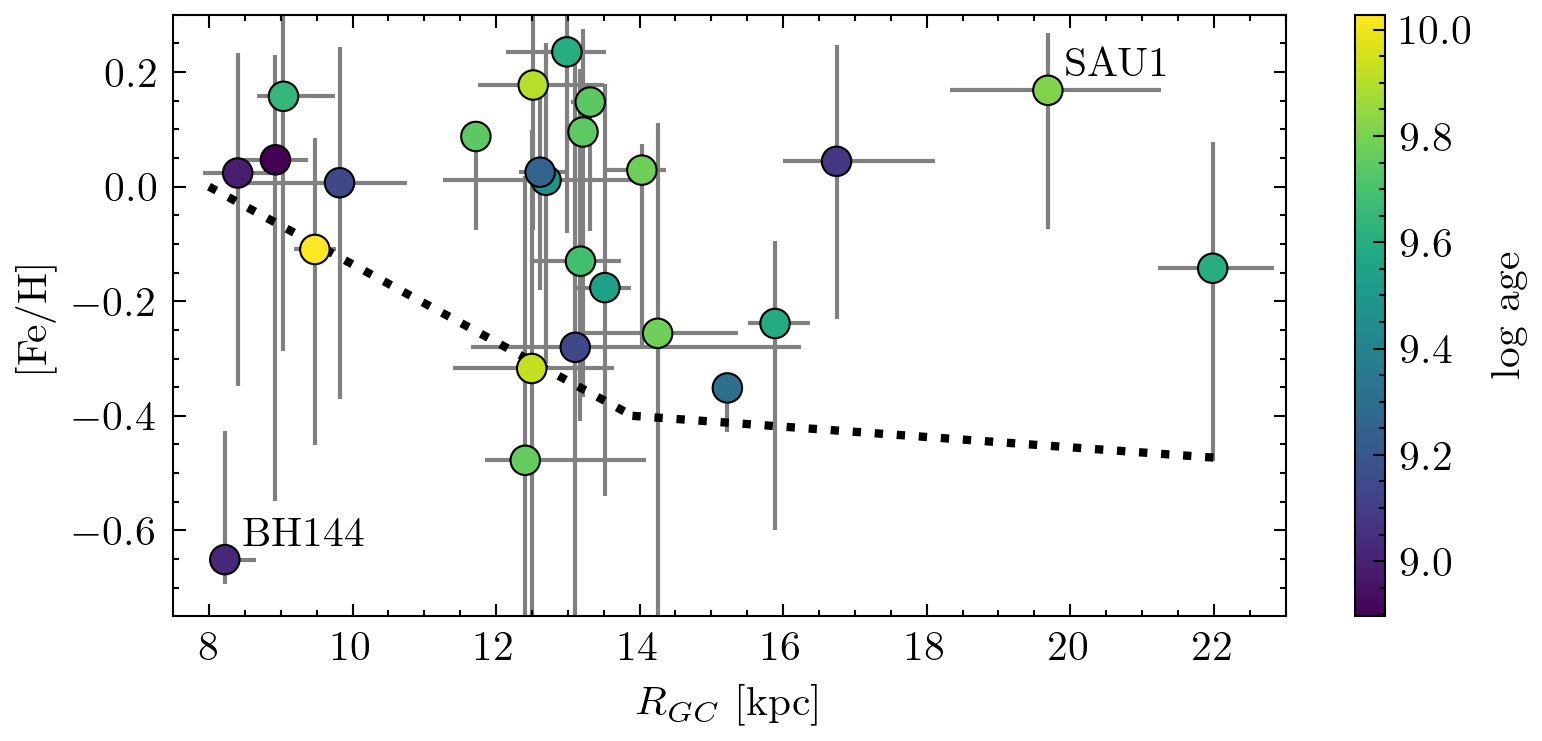
\includegraphics[]{figs/Fe_H.png}}
   \caption{Metallicity gradient for the set of twenty-five analyzed clusters.
   Points are colored according to the $\log(age)$. Grey vertical lines are the
   16th and 84th percentiles. The dotted line is the broken relation from 
   \citet[][Fig 7]{Donor_2020}.}
   \label{fig:met_gradient}
  \end{figure}






% =============================================================================
\section{Conclusions}
 \label{sec:conclusions}

 xxxxx




   %--------------------------------------------------- One column table
%    \begin{table}
%       \caption[]{Opacity sources.}
%          \label{KapSou}
%      $$ 
%          \begin{array}{p{0.5\linewidth}l}
%             \hline
%             \noalign{\smallskip}
%             Source      &  T / {[\mathrm{K}]} \\
%             \noalign{\smallskip}
%             \hline
%             \noalign{\smallskip}
%             Yorke 1979, Yorke 1980a & \leq 1700^{\mathrm{a}}     \\
% %           Yorke 1979, Yorke 1980a & \leq 1700             \\
%             Kr\"ugel 1971           & 1700 \leq T \leq 5000 \\
%             Cox \& Stewart 1969     & 5000 \leq             \\
%             \noalign{\smallskip}
%             \hline
%          \end{array}
%      $$ 
%    \end{table}



%                                                One column figure
%----------------------------------------------------------------- 
% \begin{figure}
% \centering
% %%%\includegraphics[width=3cm]{empty.eps}
%    \caption{Vibrational stability equation of state
%             $S_{\mathrm{vib}}(\lg e, \lg \rho)$.
%             $>0$ means vibrational stability.
%            }
%       \label{FigVibStab}
% \end{figure}

\section{Conclusions}

xxx

\begin{acknowledgements}
This work has made use of data from the European Space Agency (ESA) mission
{\it Gaia} (\url{https://www.cosmos.esa.int/gaia}), processed by the {\it Gaia}
Data Processing and Analysis Consortium (DPAC,
\url{https://www.cosmos.esa.int/web/gaia/dpac/consortium}). Funding for the DPAC
has been provided by national institutions, in particular the institutions
participating in the {\it Gaia} Multilateral Agreement.
%
This research has made use of the WEBDA database, operated at the Department of
Theoretical Physics and Astrophysics of the Masaryk University.
%
This research has made use of the VizieR catalog access tool, operated at CDS,
Strasbourg, France~\citep{Ochsenbein_2000}.
%
This research has made use of ``Aladin sky atlas'' developed at
CDS, Strasbourg Observatory, France~\citep{Bonnarel2000,Boch2014}.
%
This research has made use of NASA's Astrophysics Data System.
%
This research made use of the Python language v3.7.3~\citep{vanRossum_1995}
and the following packages:
NumPy\footnote{\url{http://www.numpy.org/}}~\citep{vanDerWalt_2011};
SciPy\footnote{\url{http://www.scipy.org/}}~\citep{Jones_2001};
Astropy\footnote{\url{http://www.astropy.org/}}, a community-developed core
Python package for Astronomy \citep{Astropy_2013};
matplotlib\footnote{\url{http://matplotlib.org/}}~\citep{hunter_2007}
\end{acknowledgements}




\bibliographystyle{aa}
\bibliography{biblio} % your references Yourfile.bib


% \begin{appendix}
% \section{Structure analysis}

%  \begin{figure*}
%   \resizebox{\hsize}{!}{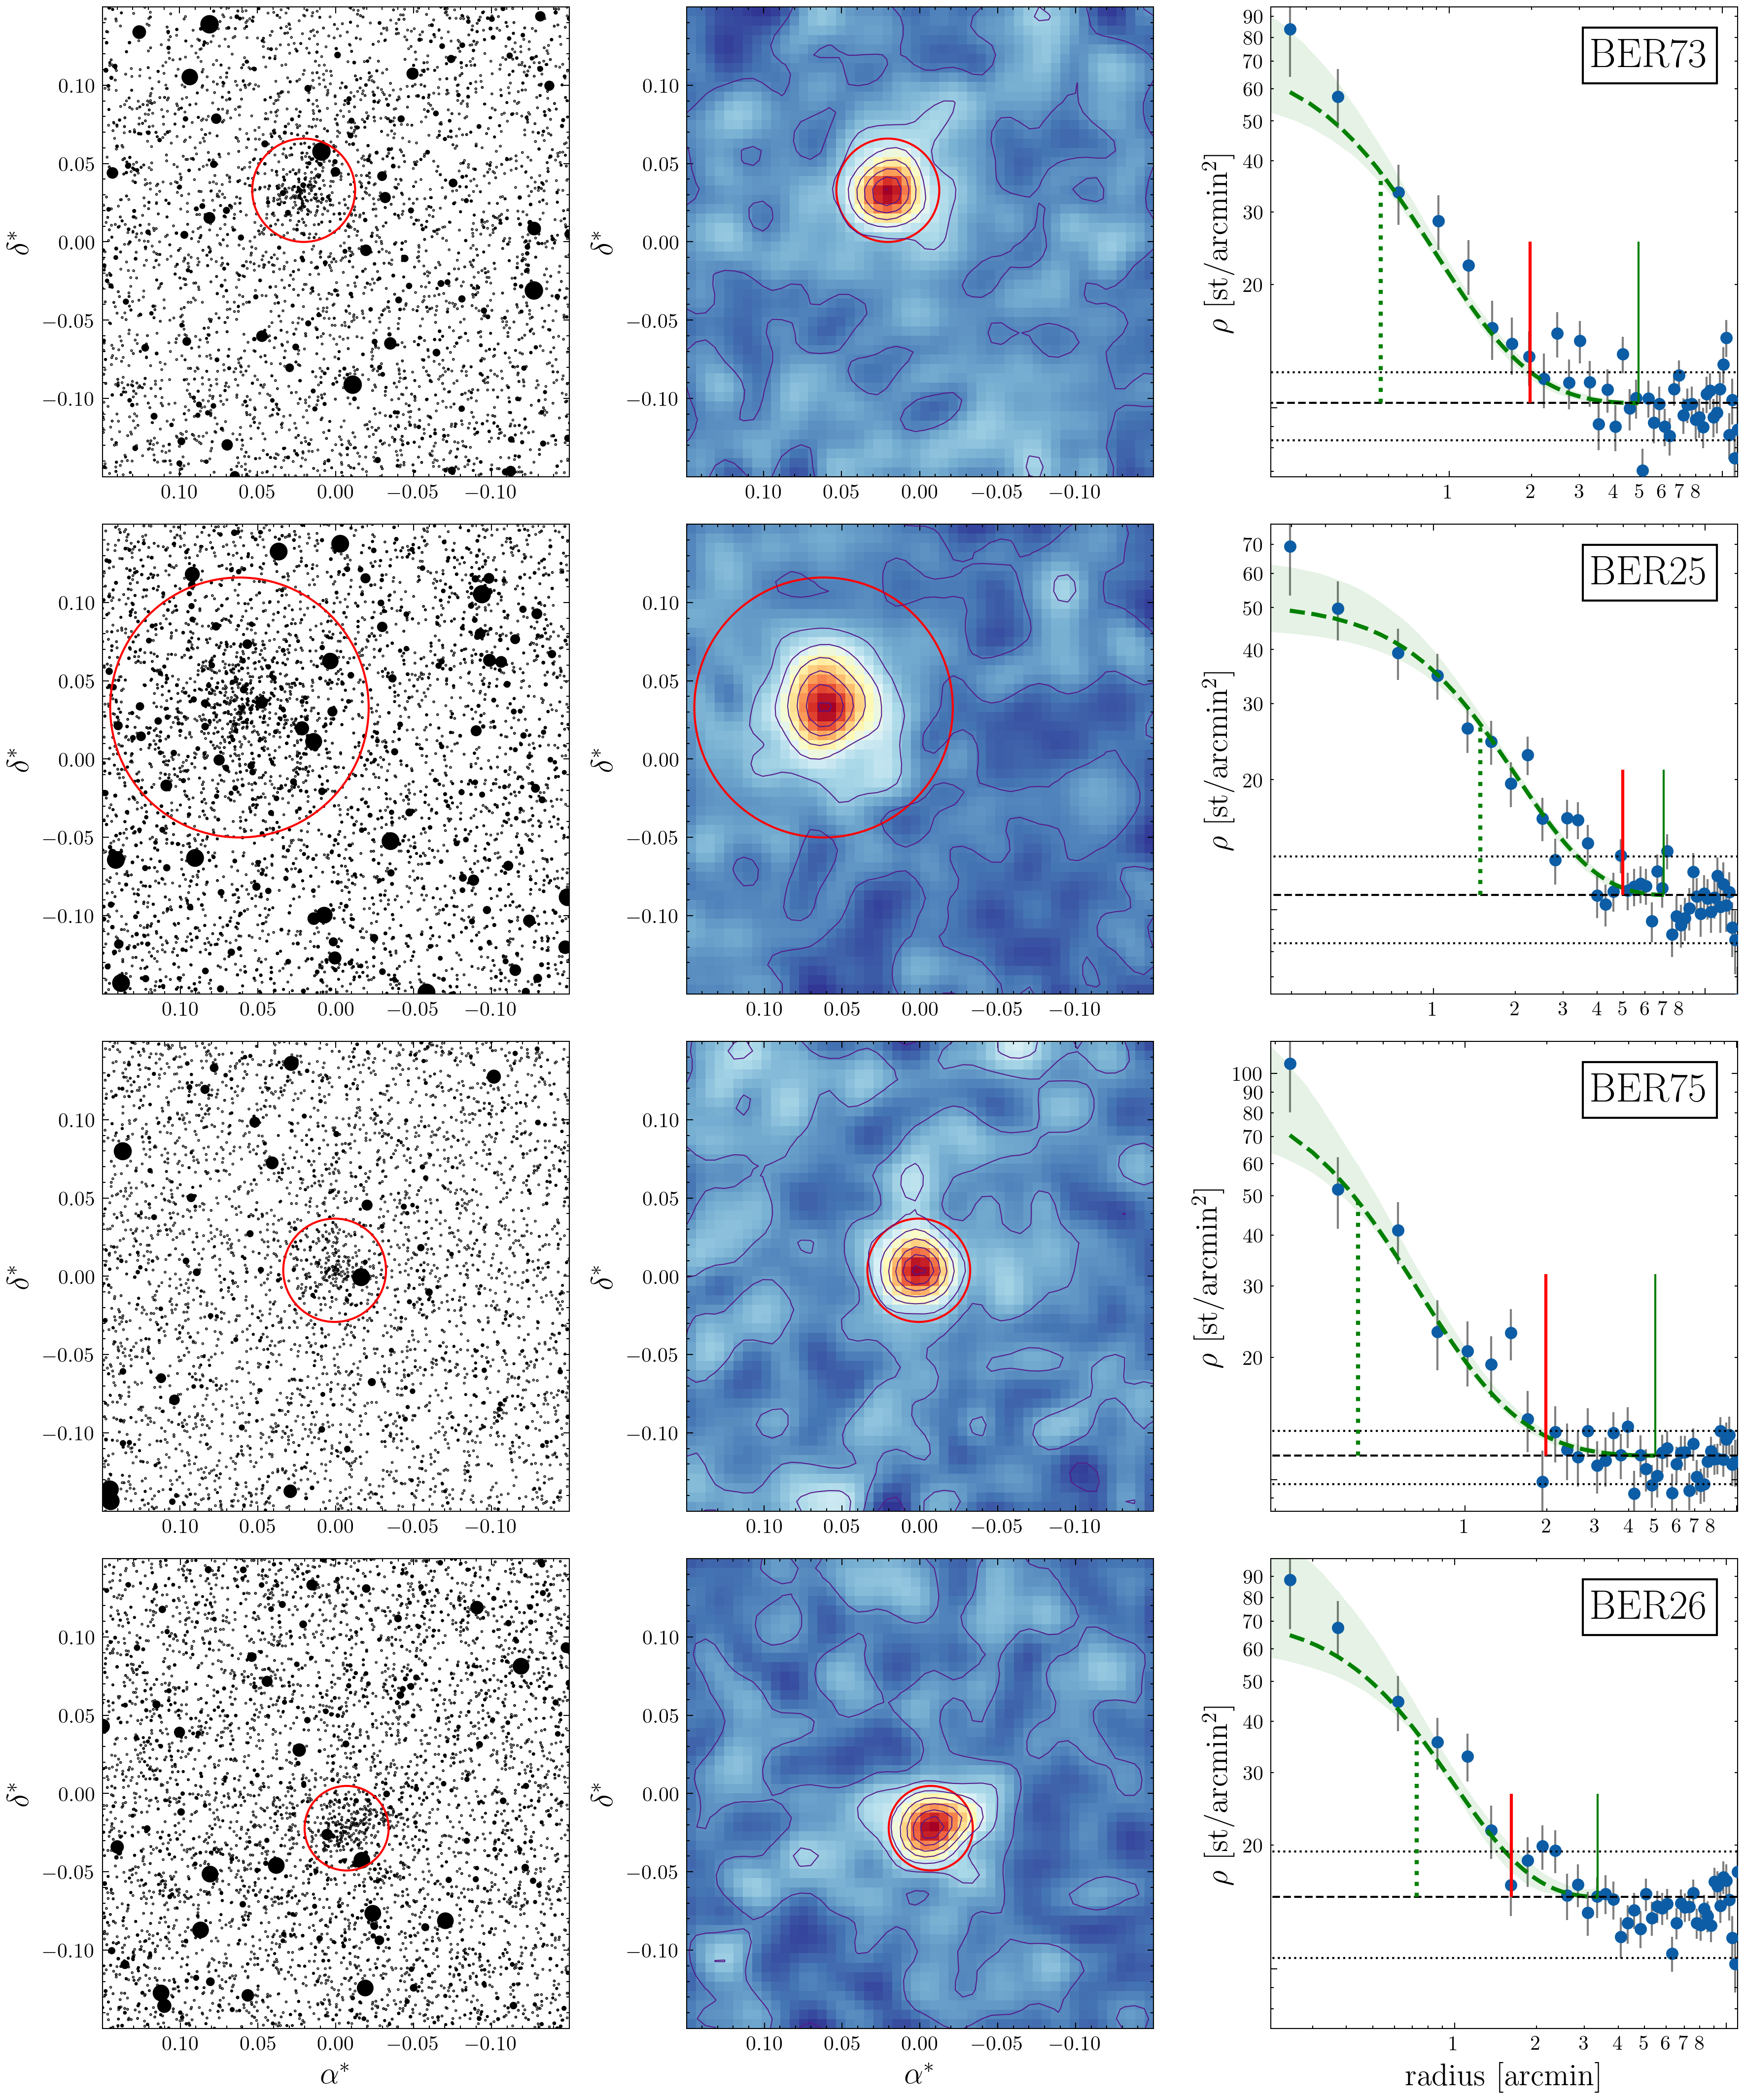
\includegraphics[]{figs/0_struct.png}}
%   \caption{xxx}
%   \label{fig:0struct}
%  \end{figure*}

%  \begin{figure*}
%   \resizebox{\hsize}{!}{\includegraphics[]{figs/4_struct.png}}
%   \caption{xxx}
%   \label{fig:4struct}
%  \end{figure*}

%  \begin{figure*}
%   \resizebox{\hsize}{!}{\includegraphics[]{figs/8_struct.png}}
%   \caption{xxx}
%   \label{fig:4struct}
%  \end{figure*}

%  \begin{figure*}
%   \resizebox{\hsize}{!}{\includegraphics[]{figs/12_struct.png}}
%   \caption{xxx}
%   \label{fig:12struct}
%  \end{figure*}

%  \begin{figure*}
%   \resizebox{\hsize}{!}{\includegraphics[]{figs/16_struct.png}}
%   \caption{xxx}
%   \label{fig:16struct}
%  \end{figure*}

%  \begin{figure*}
%   \resizebox{\hsize}{!}{\includegraphics[]{figs/20_struct.png}}
%   \caption{xxx}
%   \label{fig:20struct}
%  \end{figure*}

% \end{appendix}

\end{document}


